\chapter{Resultados e Discussões}\label{ch:discussion}

Os experimentos foram realizados com a base de dados organizada como descrita no Capítulo \ref{ch:data_preparation}. Os experimentos foram feitos com o apoio da ferramenta \textit{Scikit-Learn} que possui a implementação de diversos algoritmos de aprendizado de máquina e agrupamento, dentre eles K-Médias, que já foi discutido no capítulo 3. Também foi utilizado o pacote \textit{NumPy}, que é uma ferramenta para cálculos matriciais.

Para a preparação das análises foi adicionado ao banco de dados o registro de atividades do servidor DNS do IME de 12 de março de 2012. Nesse registro de atividades há rastros de 3 clientes suspeitos já confirmados como parte integrante de botnets através de inspeções manuais feitas na época que levaram a criação da lista de suspeitos na figura \ref{fig:suspects}.

\begin{figure}[htbp]
\centering
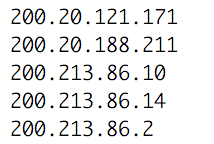
\includegraphics[scale=0.7]{ip_suspects}
\caption[Lista de IPs Suspeitos Detectados Manualmente na Base de Dados]{Lista de IPs Suspeitos Detectados Manualmente na Base de Dados} \label{fig:suspects}
\end{figure}

Foi realizada a comparação da qualidade da saída do algoritmo para dados normalizados e não normalizados. Para normalizar foi utilizada a forma \ref{eq:norm}

\begin{equation} \label{eq:norm}
\frac{\mathbf{X} - \mathbf{\bar{X}}}{\sigma}
\end{equation}

\section{Análise do Número de Grupos}

Para o cálculo da distribuição da função custo em relação ao número de grupos, apresentado na figura \ref{fig:cost_per_k}, foram criados 10 modelos para cada quantidade de centroides e calculou-se a média das funções de custos dentre cada quantidade de centroide. Esse procedimento é realizado para estabilizar os valores da função custo, já que a função custo pode estar sujeita a flutuação, por outro lado isso não pareceu crítico para esse conjunto de dados.

\begin{figure}[htbp]
\centering
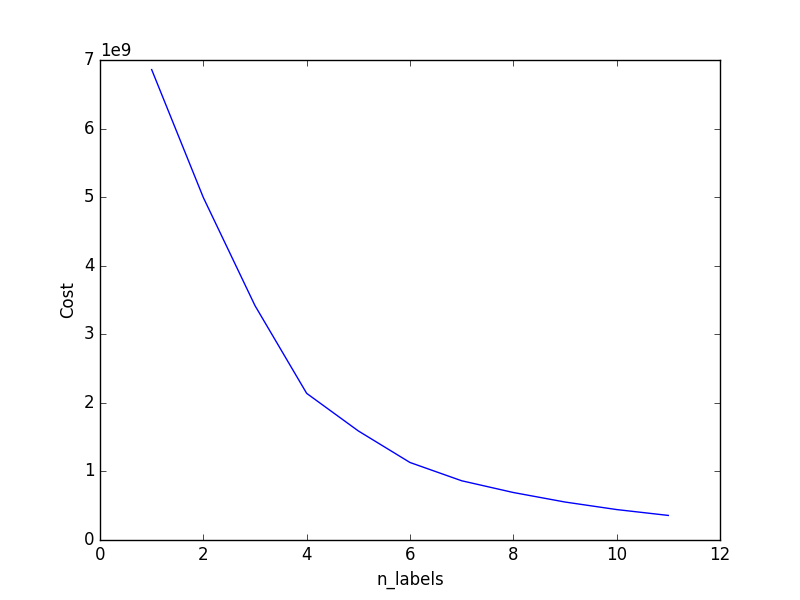
\includegraphics[scale=0.7]{cost_per_k}
\caption[Custo pelo Número de Centroides para Dados Normalizados]{Custo pelo Número de Centroides para Dados Normalizados} \label{fig:cost_per_k}
\end{figure}

Percebe-se certa ambiguidade quanto ao ponto crítico, mas é possível notar uma leve variação de curvatura no ordenada 4.

\section{Análise da Base de Dados}
\label{sec:db_analysis}

Utilizando-se 4 centroides como parâmetro, foram realizadas análises da eficácia do algoritmo de agrupamento ao conjunto de exemplos contidos no banco de dados. Em todos os experimentos o sistema consulta a tabela \textit{clients} do banco de dados e retorna na saída padrão a cardinalidade de cada grupo e os IPs das máquinas no menor grupo.

A primeira análise foi realizada observando os seguintes campos:

\begin{itemize}
\item \textit{count\_domain\_with\_numbers, }
\item \textit{average\_domain\_length, }
\item \textit{std\_domain\_length, }
\item \textit{count\_request, }
\item \textit{average\_requisition\_degree, }
\item \textit{std\_requisition\_degree e }
\item \textit{minimum\_requisition\_degree }
\end{itemize}

Os dados foram fornecidos ao algoritmo sem nenhum tratamento posterior, já que os dados já foram tratados previamente. Como resultado obteve-se a saída representada na figura \ref{fig:first_out}. Esse resultado não foi considerado um sucesso, pois o menor grupo não continha nenhum dos 3 suspeitos conhecidos, porém já apresenta um grupo de cardinalidade reduzida conforme era esperado.

\begin{figure}[htbp]
\centering
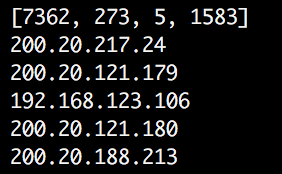
\includegraphics[scale=0.7]{first_out}
\caption[Resultado do Experimento não Normalizado]{Resultado do Experimento não Normalizado} \label{fig:first_out}
\end{figure}

Para a segunda análise, foi efetuada a normalização das características, para que cada uma tivesse o mesmo impacto para as distâncias utilizadas no algoritmo, independente do intervalo para os valores de cada uma. Após essa alteração, observou-se a saída mostrada na Figura \ref{fig:second_out}. Esse foi considerado um resultado bastante satisfatório, já que duas máquinas já confirmadas como pertencentes a botnets foram detectadas no menor grupo, cujos endereços de IP são \textit{200.213.86.2} e \textit{200.213.86.14}.

\begin{figure}[htbp]
\centering
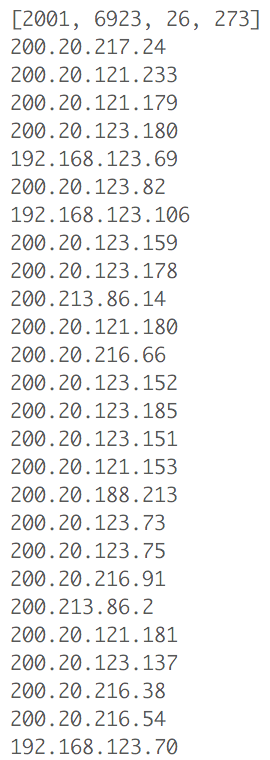
\includegraphics[scale=0.7]{second_out}
\caption[Resultado do Experimento Normalizado]{Resultado do Experimento Normalizado} \label{fig:second_out}
\end{figure}

A hipótese que se levanta para explicar o sucesso é que apesar de as máquinas com comportamento suspeito divergirem das outras máquinas, por exemplo em quantidade de requisição, a distância marginal entre elas é grande o suficiente para confundir o algoritmo ao tentar agrupa-los.

Além disso observou-se que, ao ser descartado, o campo \textit{std\_requisition\_degree} não influenciou na identificação dos itens do menor grupo, isto é, os mesmos 26 elementos permanecem consistentemente no mesmo grupo. Isso reforça a necessidade de ser aplicada uma técnica para realizar a seleção das melhores características.